%%
%% This is file `sample-sigconf.tex',
%% generated with the docstrip utility.
%%
%% The original source files were:
%%
%% samples.dtx  (with options: `sigconf')
%% 
%% IMPORTANT NOTICE:
%% 
%% For the copyright see the source file.
%% 
%% Any modified versions of this file must be renamed
%% with new filenames distinct from sample-sigconf.tex.
%% 
%% For distribution of the original source see the terms
%% for copying and modification in the file samples.dtx.
%% 
%% This generated file may be distributed as long as the
%% original source files, as listed above, are part of the
%% same distribution. (The sources need not necessarily be
%% in the same archive or directory.)
%%
%% The first command in your LaTeX source must be the \documentclass command.
\documentclass[sigconf]{acmart}
\settopmatter{printacmref=false} % Removes citation information below abstract
\renewcommand\footnotetextcopyrightpermission[1]{} % removes footnote with conference information in first column
\pagestyle{plain} % removes running headers

\usepackage{subcaption}


%%
%% \BibTeX command to typeset BibTeX logo in the docs
\AtBeginDocument{%
  \providecommand\BibTeX{{%
    \normalfont B\kern-0.5em{\scshape i\kern-0.25em b}\kern-0.8em\TeX}}}

%% Rights management information.  This information is sent to you
%% when you complete the rights form.  These commands have SAMPLE
%% values in them; it is your responsibility as an author to replace
%% the commands and values with those provided to you when you
%% complete the rights form.
%\setcopyright{none}
% \copyrightyear{}
 %\acmYear{}
 %\acmDOI{}

%% These commands are for a PROCEEDINGS abstract or paper.
%\acmConference[]{}
 %\acmBooktitle{}
% \acmPrice{}
 %\acmISBN{}


%%
%% Submission ID.
%% Use this when submitting an article to a sponsored event. You'll
%% receive a unique submission ID from the organizers
%% of the event, and this ID should be used as the parameter to this command.
%%\acmSubmissionID{123-A56-BU3}

%%
%% The majority of ACM publications use numbered citations and
%% references.  The command \citestyle{authoryear} switches to the
%% "author year" style.
%%
%% If you are preparing content for an event
%% sponsored by ACM SIGGRAPH, you must use the "author year" style of
%% citations and references.
%% Uncommenting
%% the next command will enable that style.
%%\citestyle{acmauthoryear}

%%
%% end of the preamble, start of the body of the document source.

\begin{document}

%%
%% The "title" command has an optional parameter,
%% allowing the author to define a "short title" to be used in page headers.
\title{DL2021: Investigation of Image Classification based on Transfer Learning and Siamese Network}

%%
%% The "author" command and its associated commands are used to define
%% the authors and their affiliations.
%% Of note is the shared affiliation of the first two authors, and the
%% "authornote" and "authornotemark" commands
%% used to denote shared contribution to the research.
  
\author{Abdullateef Almudaifer}
\email{lateef11@uab.edu}
\affiliation{%
  \institution{University of Alabama at Birmingham}}
  
\author{Ke Fan}
\email{kefan@uab.edu}
\affiliation{%
  \institution{University of Alabama at Birmingham}}

\author{Sungman Kang}
\email{sungman@uab.edu}
\affiliation{%
  \institution{University of Alabama at Birmingham}}


%%
%% By default, the full list of authors will be used in the page
%% headers. Often, this list is too long, and will overlap
%% other information printed in the page headers. This command allows
%% the author to define a more concise list
%% of authors' names for this purpose.
%\renewcommand{\shortauthors}{Ke Fan, et al.}

%%
%% The abstract is a short summary of the work to be presented in the
%% article.
\begin{abstract}
 xxxxxxxxxxxx
\end{abstract}


\keywords{}

\maketitle

%\begin{itemize}
%\item {\verb|acmsmall|}: The default journal template style.
%\item {\verb|acmlarge|}: Used by JOCCH and TAP.
%\item {\verb|acmtog|}: Used by TOG.
%\end{itemize}

\section{Introduction}



\section{Dataset Processing}

In this project, we apply methods to the UT Zappos50K dataset \cite{yu2014fine}, which is a large shoe dataset. It collected more than 50,000 images of shoes from Zappos.com. The dataset contains four main classes, which are shoes, sandals, slippers, and boots. Each category is a sub-folder under the root directory. In each category folder, the images are divided into several sub-folders based on the functional types, followed by the individual brands. Figure \ref{fig:data_folder} shows an example of the structure of the dataset. Figure \ref{fig:data_example} illustrates the five samples in the four categories. We can observe that each image is centered on a white background and pictured in the same orientation. 

\begin{figure}[h]
	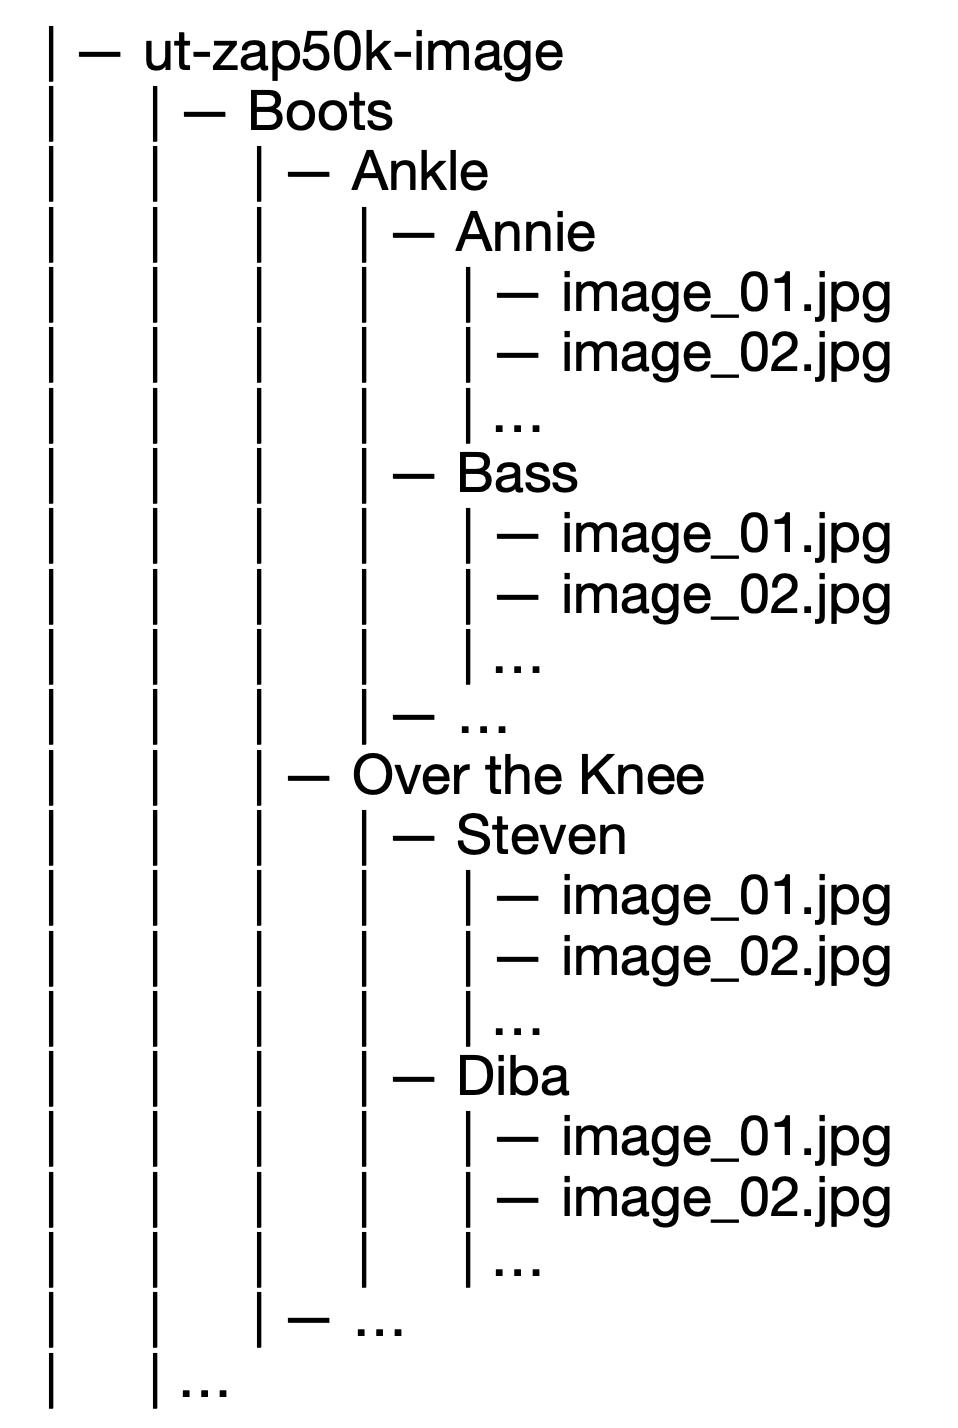
\includegraphics[width=0.5\linewidth]{figs/data_folder.png}
	\caption{An example of the folder structure of dataset }
	\label{fig:data_folder}
\end{figure}

\begin{figure}[h]
	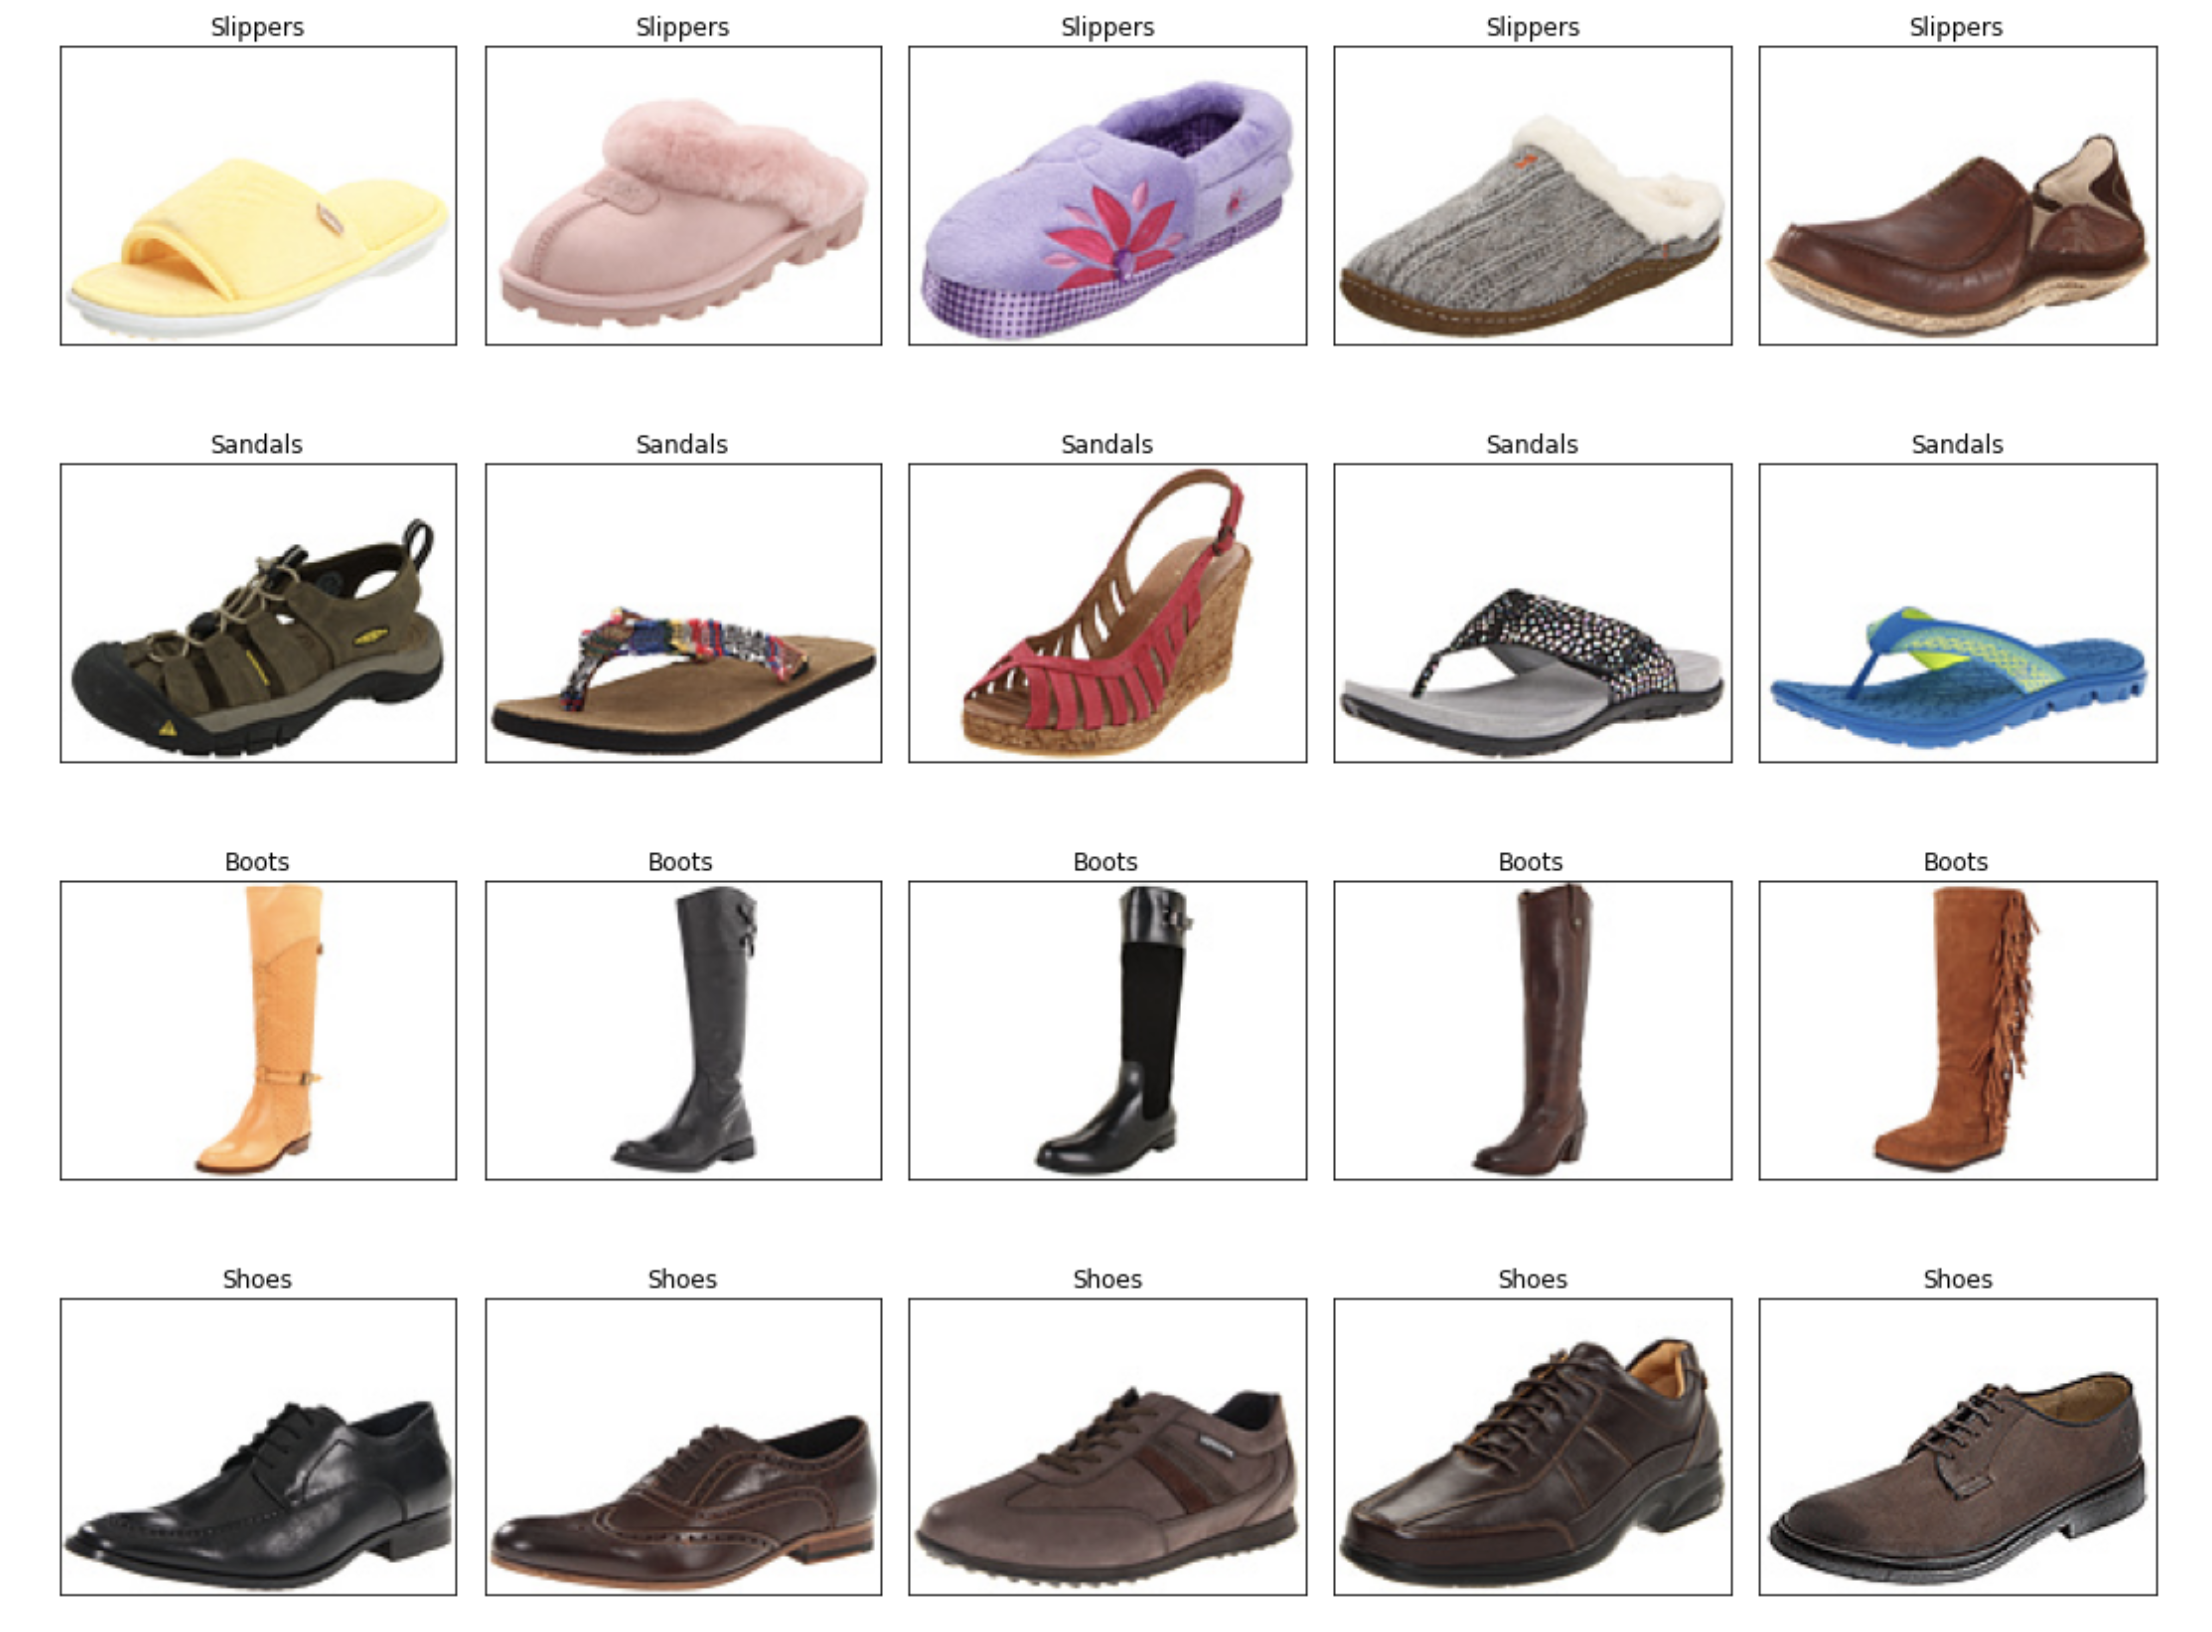
\includegraphics[width=\linewidth]{figs/data_example.png}
	\caption{An example of four categories in the dataset }
	\label{fig:data_example}
\end{figure}

\begin{table}[ht]
    \caption{Data distribution} 
    \centering 
    \begin{tabular}{c c c c} 
    \hline\hline 
    Shoes & Slippers & Sandals & Boots  \\% inserts table
    \hline % inserts single horizontal line
    30169 & 1283 & 5741 & 12832 \\% inserting body of the table
    1500 & 1283 & 1500 & 1500 \\% inserting body of the table
    2500 & 2500 & 2500 & 2500 \\% inserting body of the table
    \hline 
    \end{tabular}
\label{table:data} % is used to refer this table in the text
\end{table}

In this project, we only need the four major categories. So we merge all the images in each sub-folders, shown in figure \ref{fig:data_folder} into the category folder. In this way, we can label each image with its category folder name. Moreover, the first row of table \ref{table:data} represents the distribution of the four categories. We can see that the distribution of the dataset is very imbalanced. Especially, slippers are fewer than others. To create a balanced dataset for better accuracy calculation, we choose the first 1500 images from each category except Slippers, which use all the images. So in total, we have 5783 samples, as shown in the second row of table \ref{table:data}.

Besides, we know data argumentation such as flips, translations or rotations is good for getting more images. The ImageOps module contains some image processing operations. So we choose the mirror function, actually, it is the same as horizontal flip. In this way, we try to create a larger sub-dataset, which is shown in the third row of table, \ref{table:data} for the slippers class. In this project, we conduct an experiment to study the impact on augmenting a single class of the dataset.

On the other hand, our models implemented in this project all work well with a small dataset. Then we partition these samples into train, test, validation datasets with a ratio of 8:1:1. 



\section{Transfer Learning}

Transfer learning is when a model is train for one task and try to use that knowledge for another related task, usually within the same domain.  Figure \ref{fig:transfer} shows some intuitive examples inspired by human ability to relatively easily transfer the knowledge learned from the task on the wright of the arrows to the ones on the left. This idea have been applied to ML across all domains. In this project, we leveraged this idea by transferring the knowledge from a model that was trained on ImageNet dataset for the problem of shoes classification.

Xception \cite{chollet2017xception} was proposed in 2017 by Chollet. It is a convolutional neural network that is 126 layers deep and it was pretrained on the ImageNet dataset. The architect of this model take inspiration form Inception, but the Inception modules were replaced with depthwise separable convolutions. In-spite of the depth, this this make more efficient use of the model parameters, which even lead to better performance. Also, it is ranked the top 1 accuracy on kearas applications. Thus, it is a good fit to our problem. 

\begin{figure}[h]
  \centering
  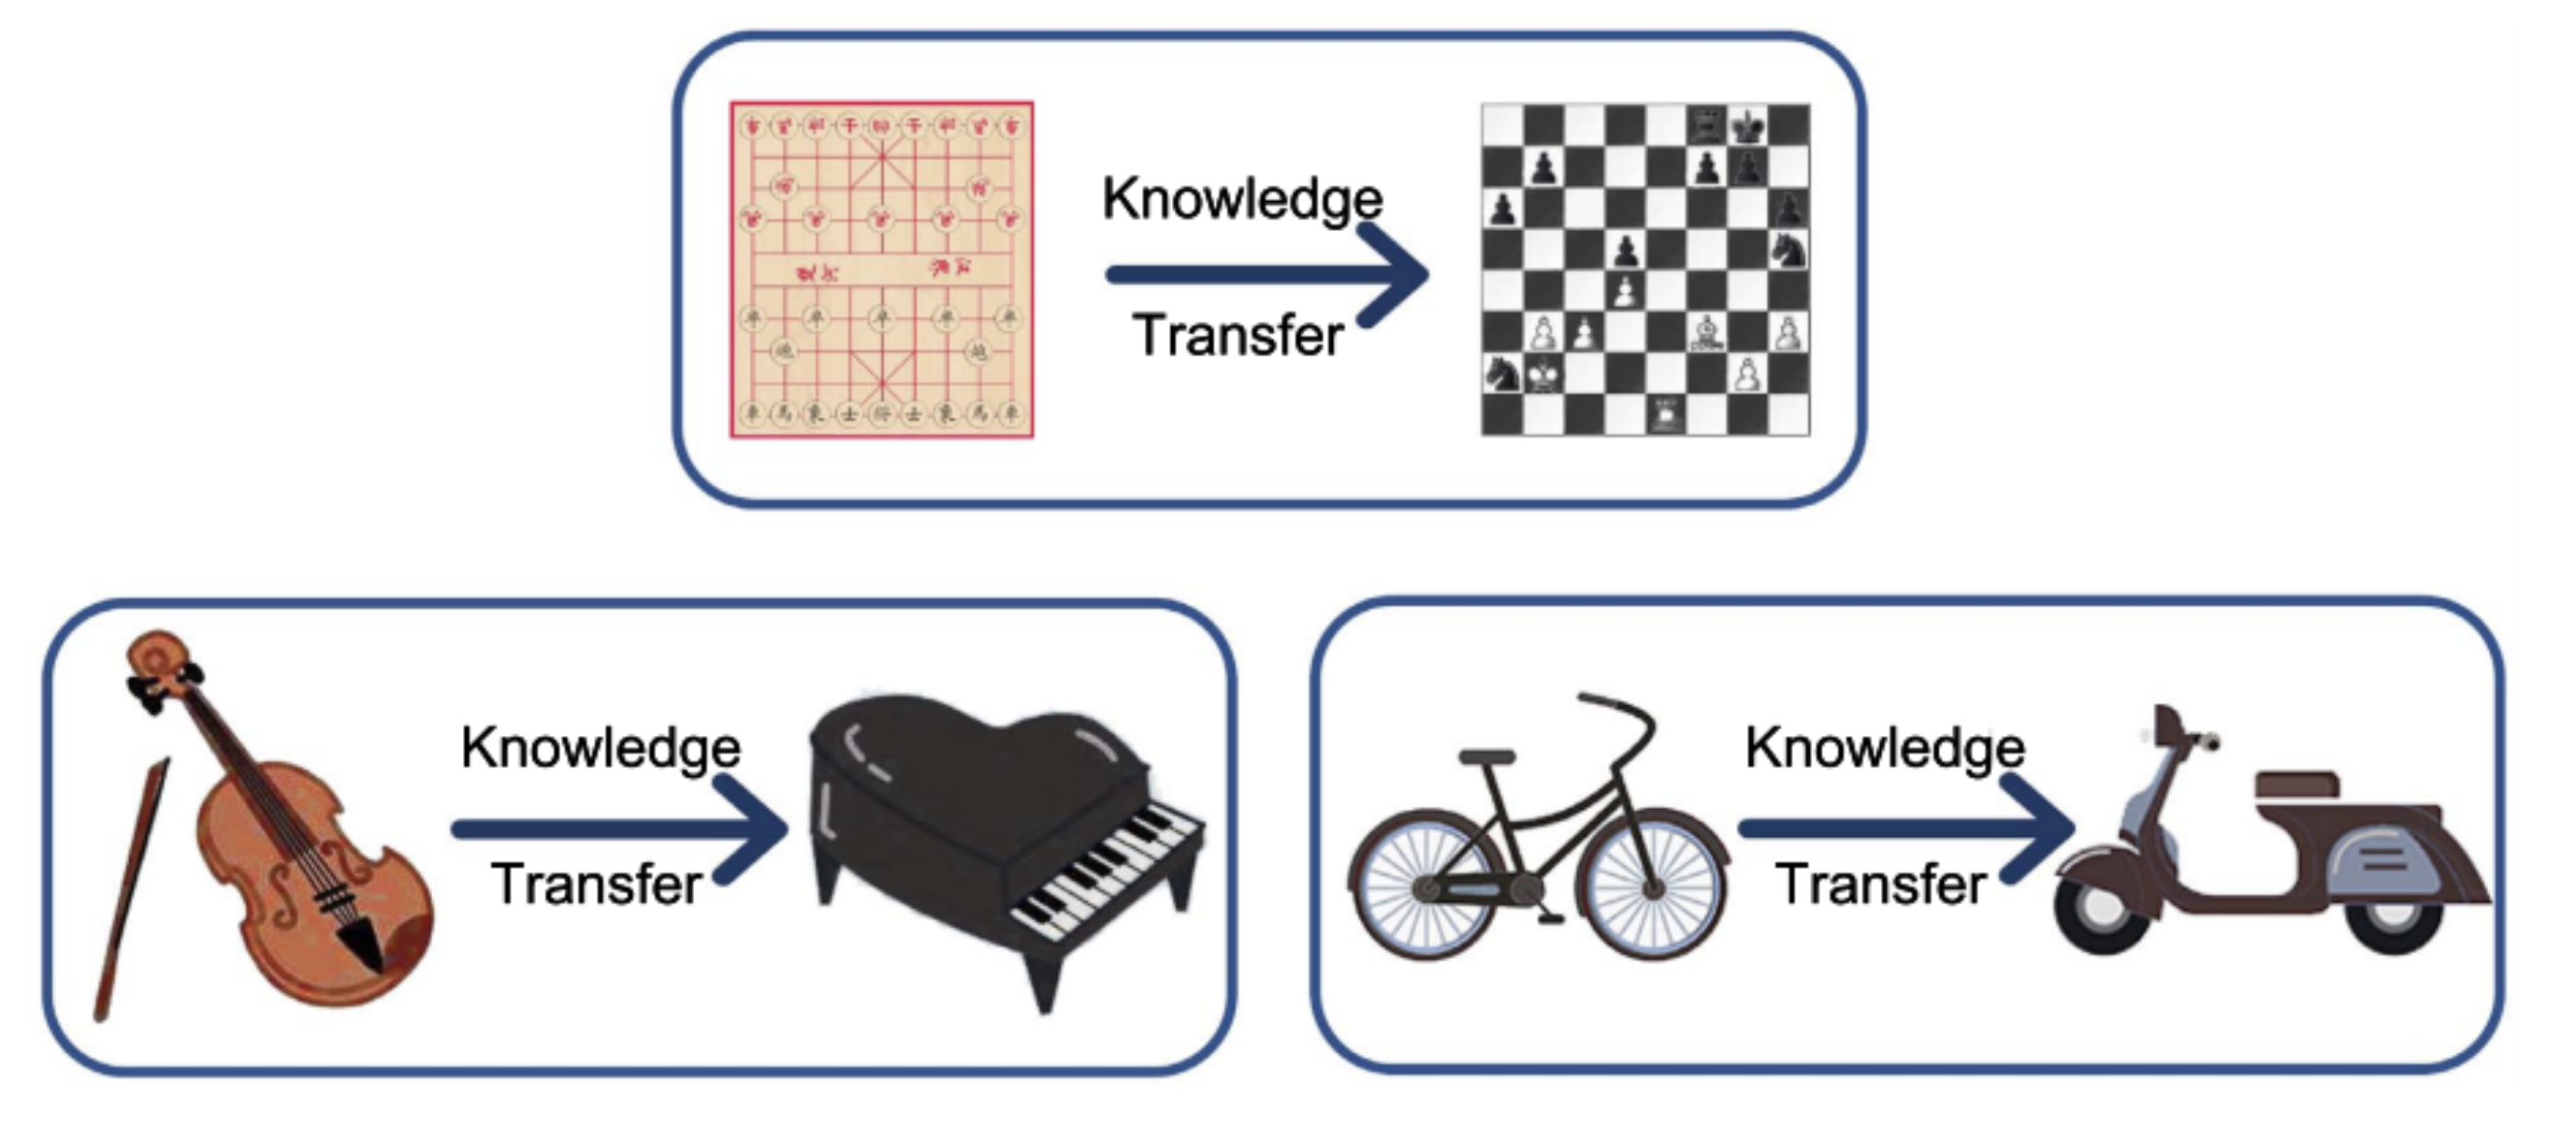
\includegraphics[width=\linewidth]{figs/transfer_learning.png}
  \caption{Intuitive examples about transfer learning.}
  \label{fig:transfer}
\end{figure}

\begin{figure}[h]
  \centering
  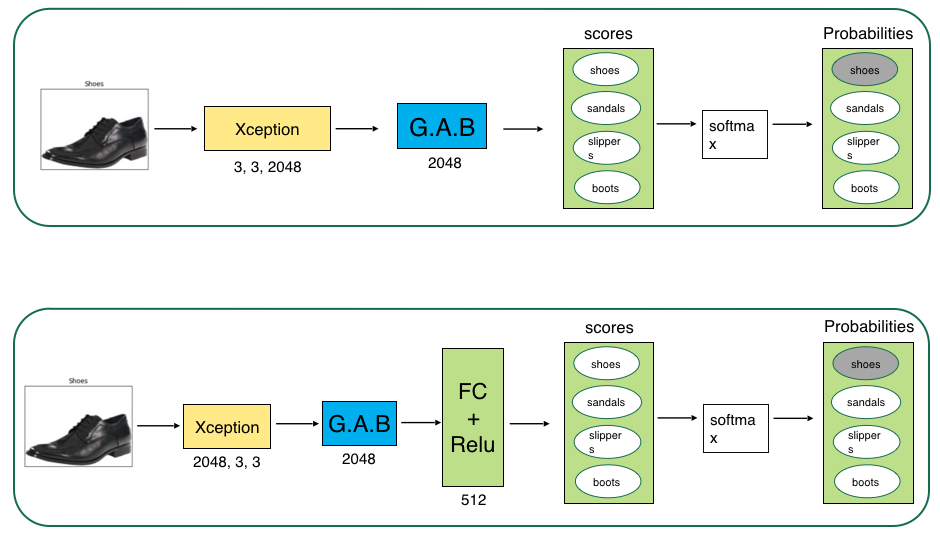
\includegraphics[width=\linewidth]{figs/xception.png}
  \caption{Transferring Xception to our image classification model.}
  \label{fig:transfer}
\end{figure}

\section{Siamese Network}

Siamese networks, first introduced by Bromley \cite{bromley1993signature} in 1993, contains multiple instances of the same model and share the same configuration and weights. The term “siamese twins,” means “conjoined twins,” which is two identical twins connected in utero. These twins share the same organs. Each sub-network is a typical Convolutional Neural Network (CNN).

The siamese networks accept distinct inputs and learn their feature vectors, joined by an energy function at the top. This function computes the similarity between the highest-level feature representation on each side. Parameter updates are mirrored across the twin networks. This means if the weights on one network are updated, then the weights on the other one are also updated. It guarantees the two similar inputs will not be mapped by each network to different locations in feature space. Furthermore, instead of training a classification model to classify the dataset into correct categories, it asks the model to recognize if the two inputs are similar or not. It means that the siamese network architectures do not need to concern themselves with classification to select 1 of N possible classes, like the traditional classification model. Rather, they only answer whether the two inputs are similar or not. Based on the characteristics, siamese networks perform well in the scenario that the dataset consists of numerous categories but in which each class has few samples. Therefore, siamese networks have been successfully applied to address face recognition \cite{schroff2015facenet}, image retrieval, person re-identification \cite{fang2019bilinear}, localization \cite{tompson2015efficient}, and even object tracing \cite{bertinetto2016fully} tasks. 

In most cases, the siamese networks have a strong embedding capability to learn a non-linear embedding of data to obtain semantically meaningful spaces. In these spaces, the related patterns of similar objects are close to each other while unrelated patterns of different objects are far away from each other. In general, the training of the siamese network is accomplished by two steps: 1) learning non-linear embeddings of inputs, 2) followed by distance-based loss functions. The loss functions usually aim at constraining the learned embeddings to have shorter distances among samples of the same category than the distances of the distinct categories \cite{medela2019constellation}. There are several widely used distance-based loss functions, contrastive loss function \cite{sohn2016improved}, triplet loss \cite{schroff2015facenet}, multiclass-N-pair loss function \cite{chopra2005learning} and so on. The objective of these loss functions is to predict the relative distance between inputs instead of directly a label or a value given an input. The contrastive loss function measures pairs of samples. The triplet loss function is extended to compare a sample with its positive and negative samples. Meanwhile, the multiclass-N-pair loss function is to improve distance loss functions by generalizing triplet loss. The distance-based loss function selection is very flexible in terms of the dataset. 

In this project, we applied the contrastive loss function and triplet loss function into siamese networks. Because they are the two most frequently used loss functions, as detailed below. 

\subsection{Contrastive Loss}
The training process with contrastive loss function is depicted in figure \ref{fig:contrastive}. The model takes image pairs as its inputs, which contain both the positive pairs and negative pairs. From the figure, it's clear that the positive pairs are composed of an anchor sample and a positive sample that is similar to the anchor. In contrast, the negative pairs contain an anchor sample and a negative sample which is dissimilar to the anchor. The objective of this model is to learn representations with a shorter distance between the positive pairs than the negative ones. Formally, the model transforms the image pairs $x_{1,i}, x_{2,i}$ into embedding vectors $v_{1,i}, v_{2,i}$, $i \in (1, N)$, where $N$ is the batch size. The contrastive loss tries to force positive pairs have 0 distance, and negative pairs have a distance greater than a margin $m$. Let $d$ be the distance function, the loss can be expressed by formula \ref{equ:loss}: 

\begin{equation}
L_i = \left\{
\begin{aligned}
 & d(v_{1,i}, v_{2,i}) \ i \in (1, N) \ \ \ \ \text{if positive pairs} \\
 & max(0, m - d(v_{1,i}, v_{2,i}) \   i \in (1, N) \ \  \  \text{if negative pairs} \\
\end{aligned}
\right.
\label{equ:loss}
\end{equation}

For positive pairs, zero loss means the model generates embeddings for both two samples with no distance between them. The loss is increased with this distance. For negative pairs, zero loss indicates that the distance between the embeddings of the two samples is larger than the margin $m$. Otherwise, the loss is a positive value and the model will update the related parameters to increase the distance for them. As shown in the figure \ref{fig:contrastive}, similar objects are pushed closer together while the dissimilar objects are push away from each other until the distance is larger than the margin $m$. From the formula, we observe that the largest loss of negative pairs is $m$ when the distance between the two samples is 0. Note that, there is no need to increase the distance between the negative pairs when it's already larger than the marge $m$. In doing so, we can save efforts to train other difficult parts. 

Assume $y_i$ is the binary label that equals 1 for a positive pair and 0 for a negative pair. And distance is the euclidian distance. The contrastive loss function is as formula \ref{equ:contrastive}.

\begin{equation}
L = \frac{1}{2N}\sum_{i=1}^{N}[y_i || v_{1,i} - v_{2,i} ||_2^2 +  (1 - y_i)\{ max(0, m - ||v_{1,i} - v_{2,i}||_2^2) \}]
\label{equ:contrastive}
\end{equation}

\begin{figure}[h]
  \centering
  \begin{subfigure}[b]{\linewidth}
  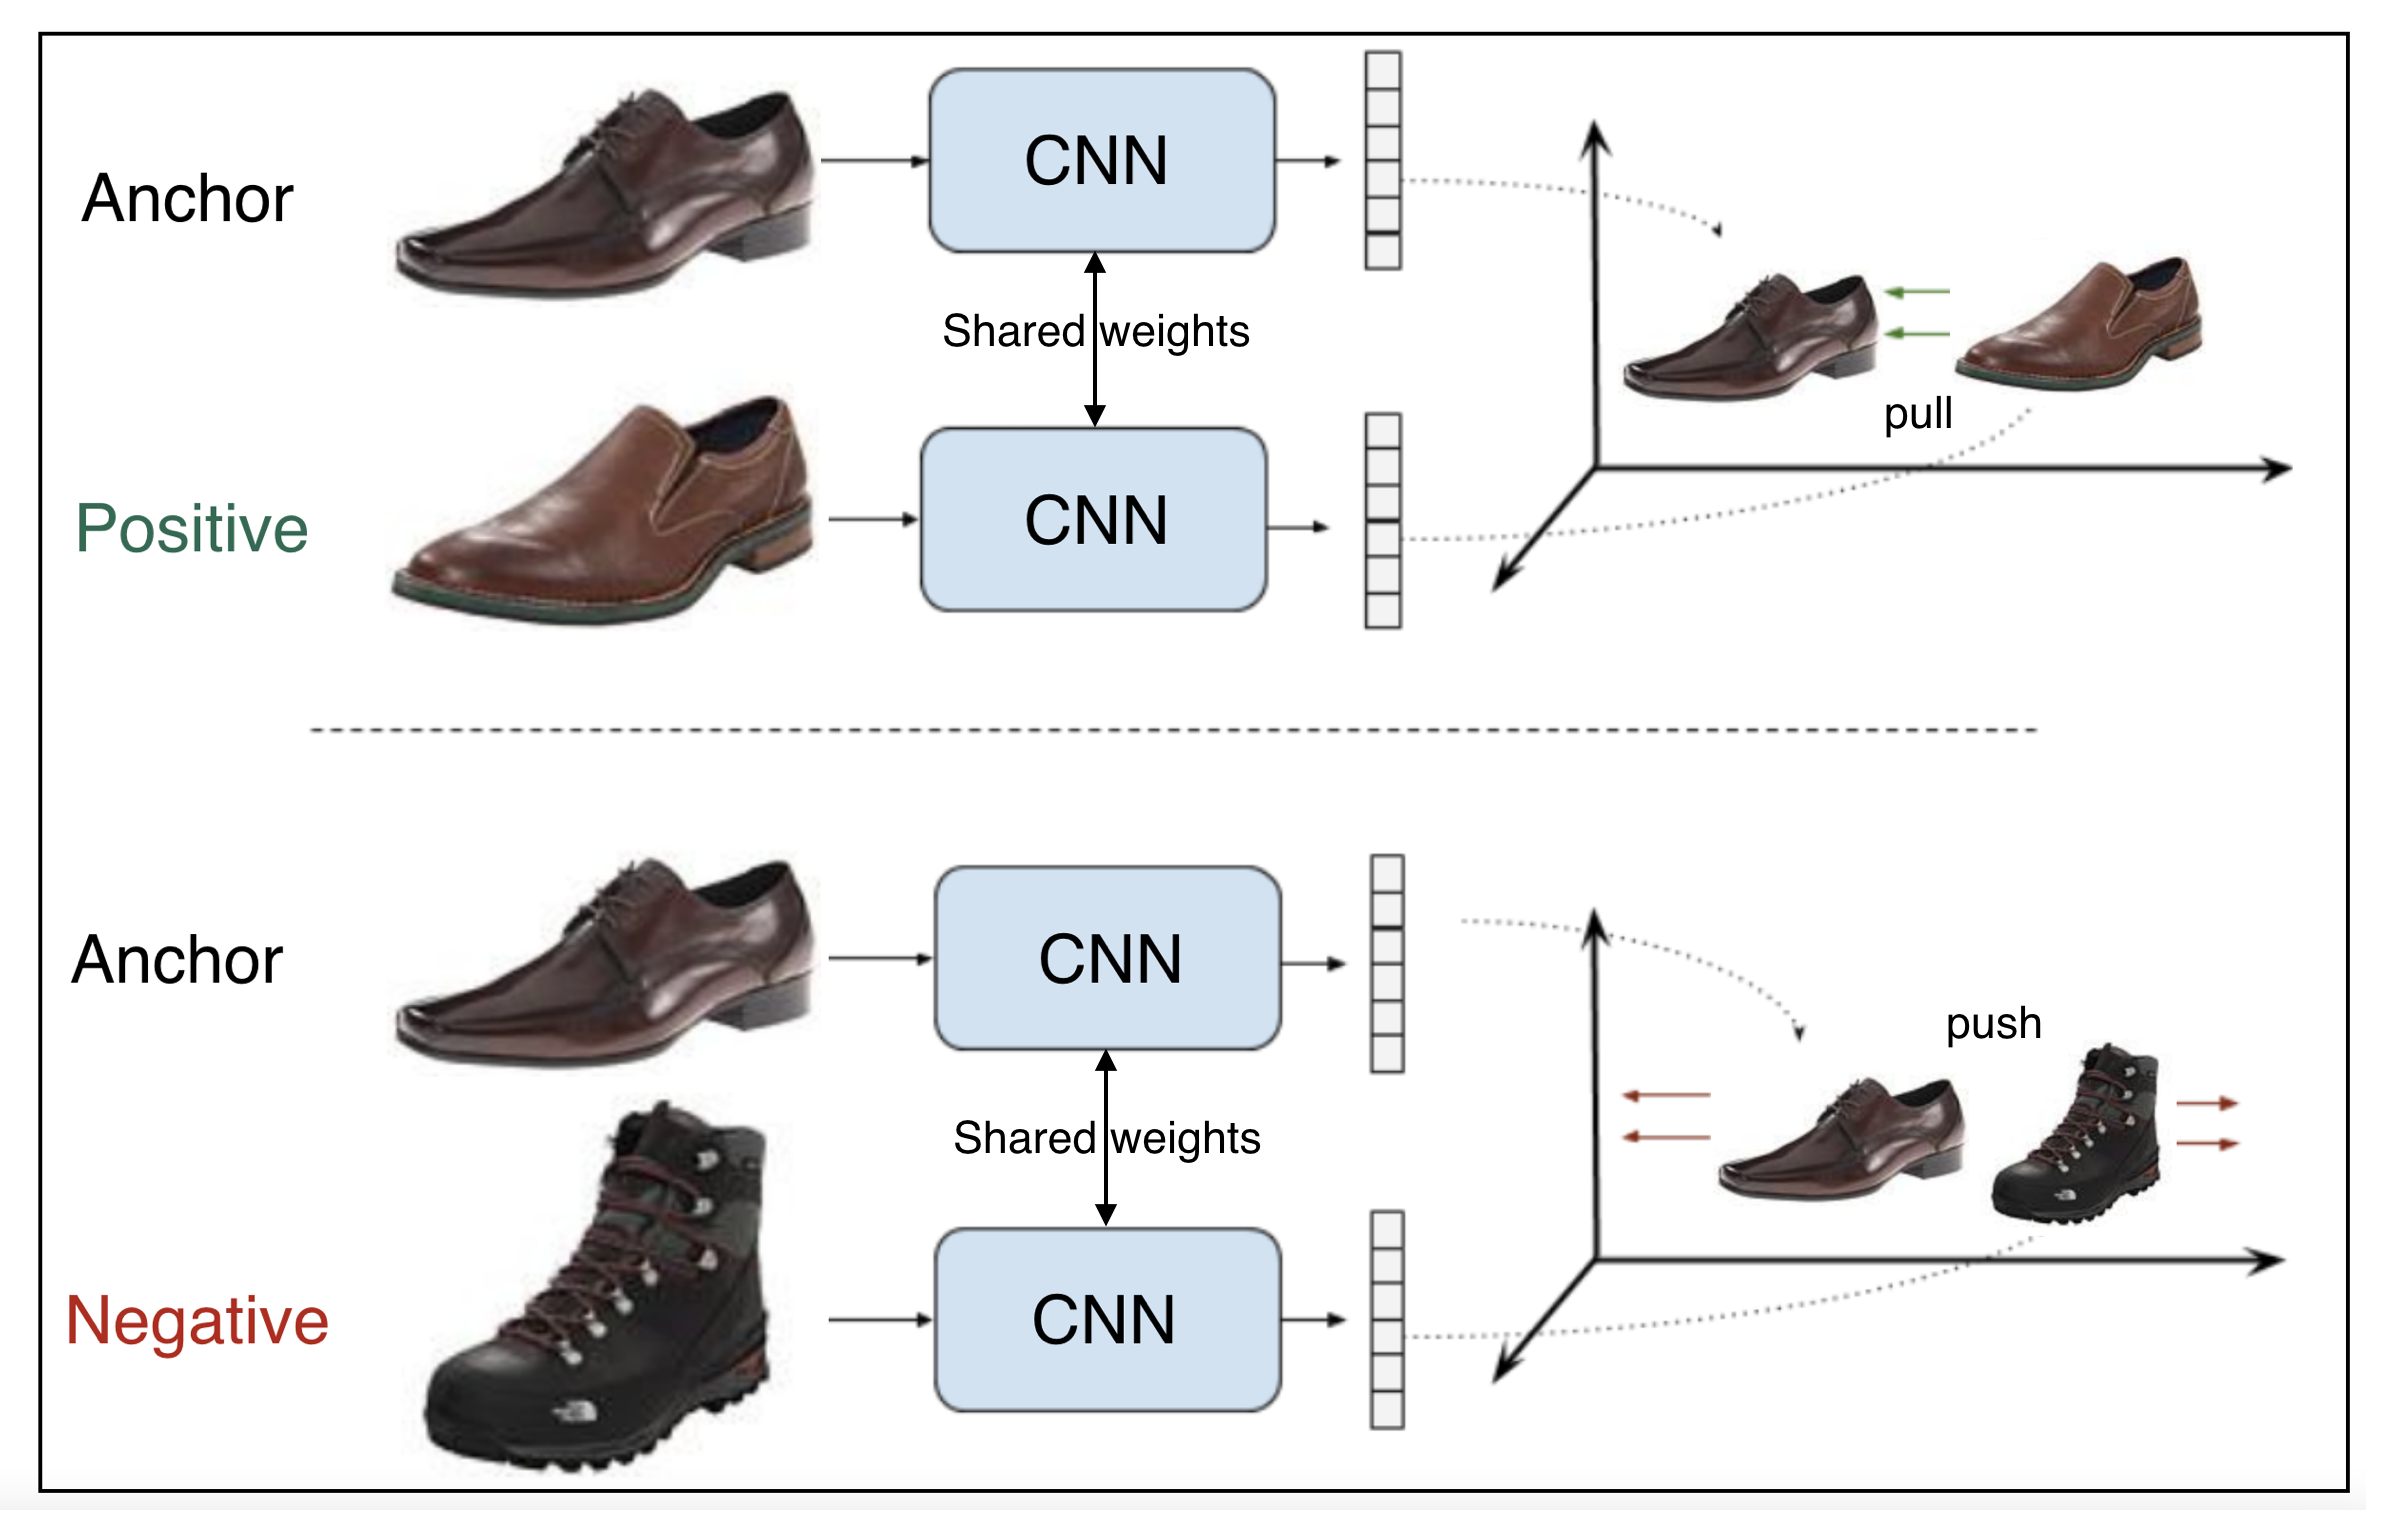
\includegraphics[width=\linewidth]{figs/contrastive.png}
  \caption{Training with contrastive loss function}
  \label{fig:contrastive}
  \end{subfigure}
  \hfill
    \begin{subfigure}[b]{\linewidth}
   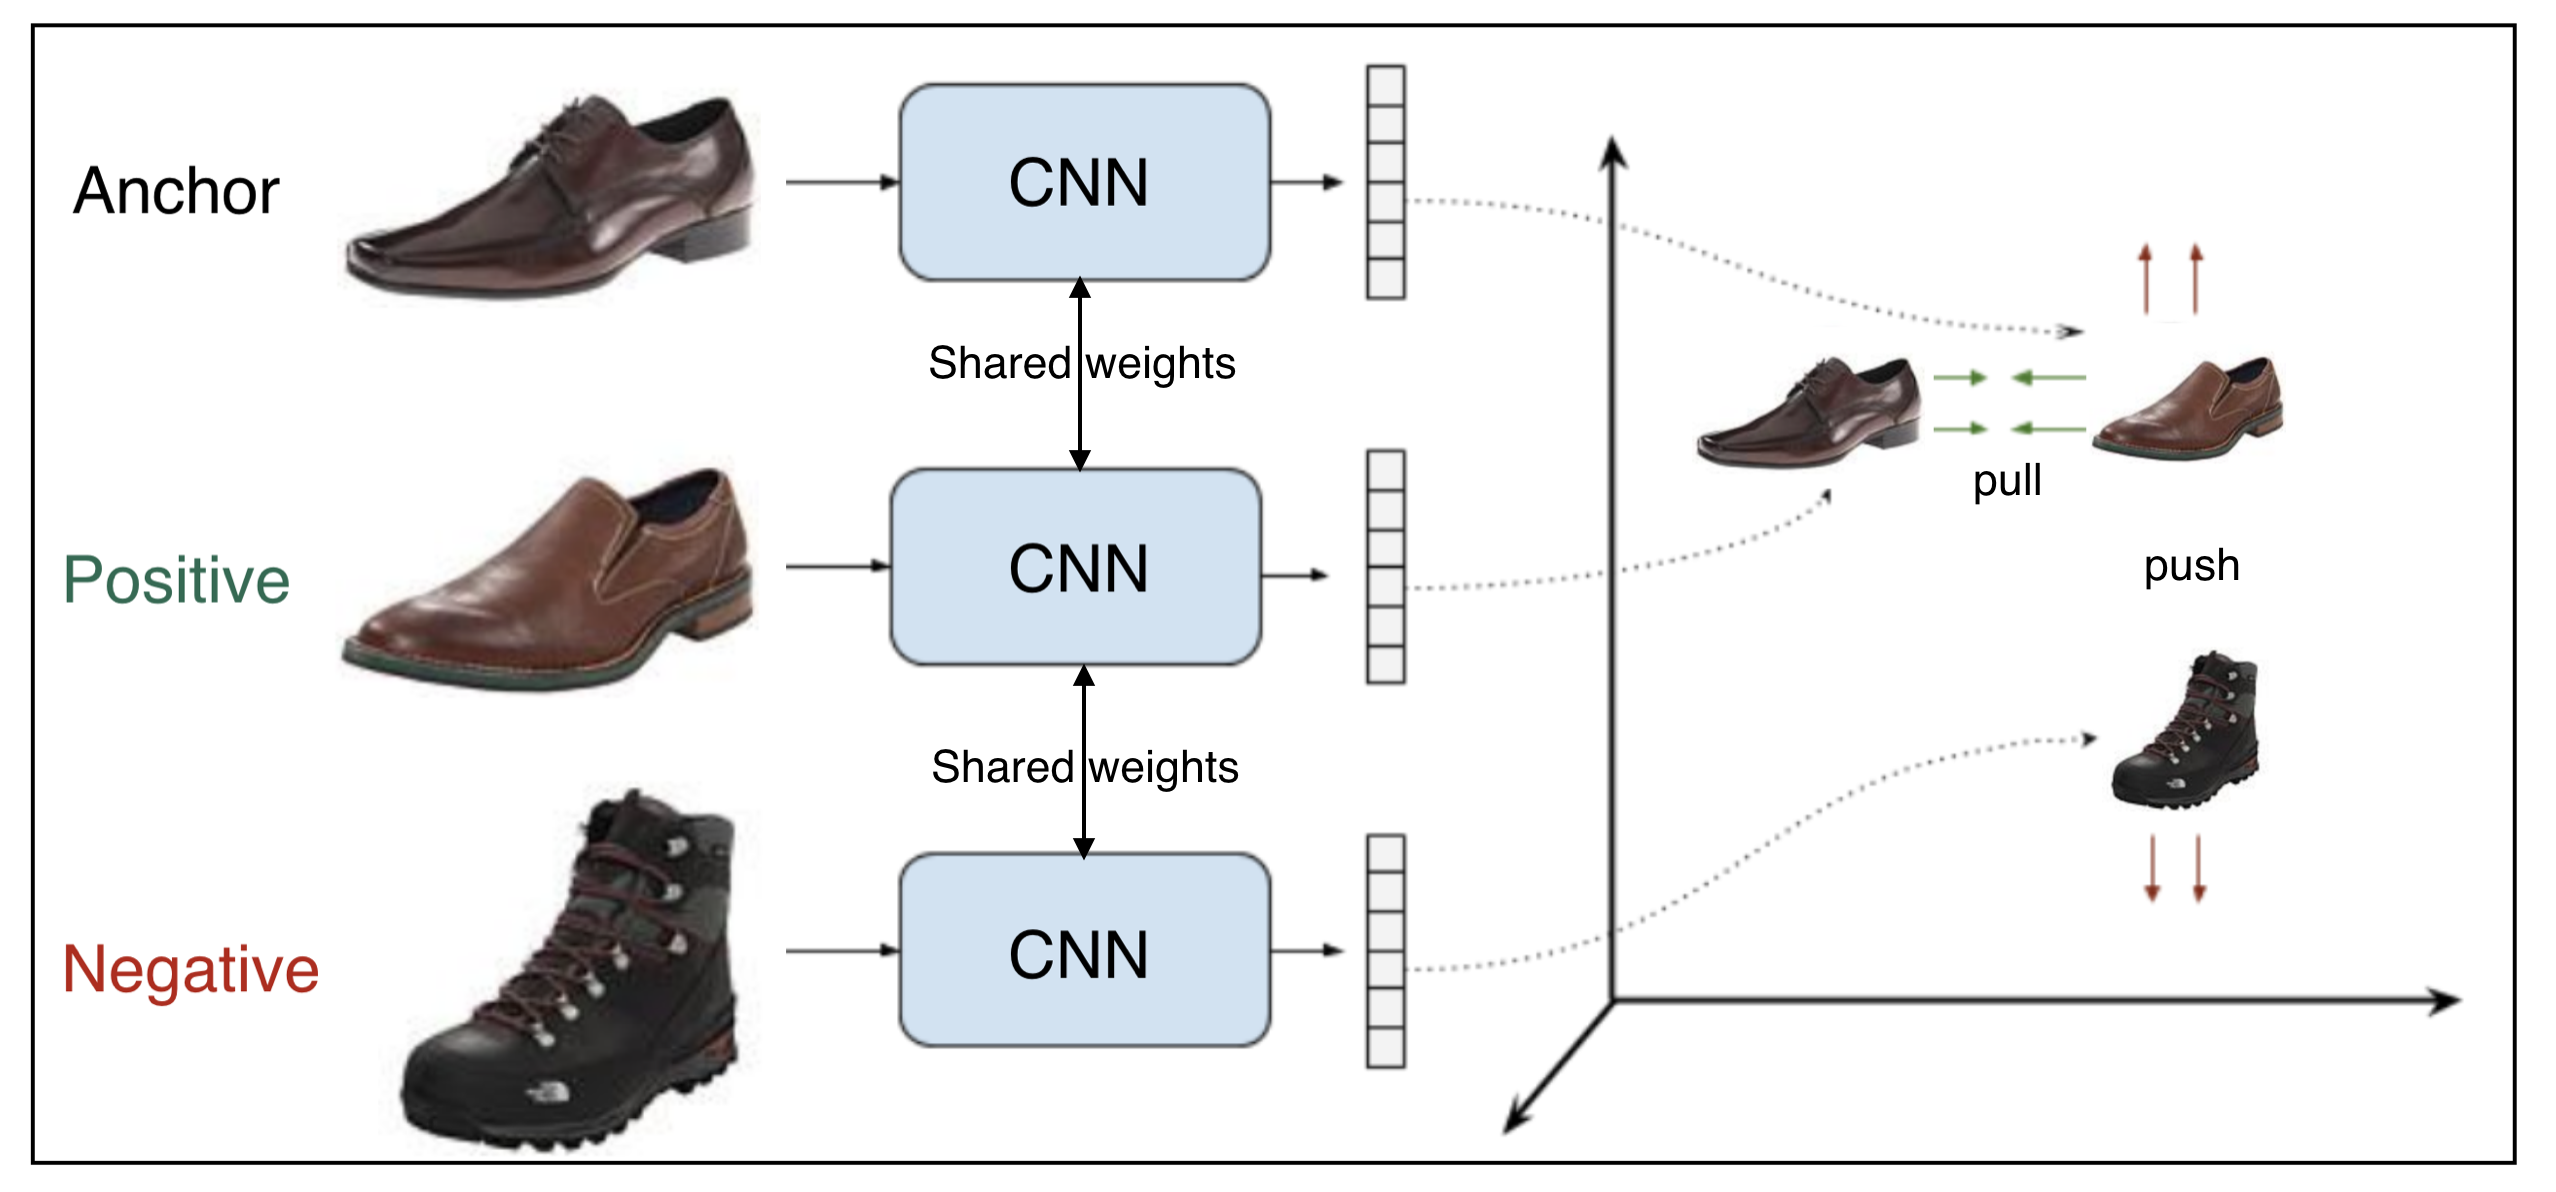
\includegraphics[width=\linewidth]{figs/triplet.png}
   \caption{Training with triplet loss function}
   \label{fig:triplet}
  \end{subfigure}
  \hfill
    \caption{Visual representation of training siamese network with different loss functions.}
    \label{fig:sialoss}
\end{figure}

\subsection{Triplet Loss}

Triplets loss function goes further by considering positive and negative pairs at the same time. The training process is shown in figure \ref{fig:triplet}. We can see that the model with triplets loss uses triplets of training samples, instead of pairs. A triplet consists of an anchor, a positive sample, and a negative sample. The goal is to minimize the distance between the anchor sample and the positive sample while maximizing the distance between the anchor sample and the negative sample. Assume $x_{a,i}, x_{p,i}, x_{n,i}$ are the anchor sample, positive sample and negative sample in a triplet respectively. $v_{a,i}, v_{p,i}, v_{n,i}$ are their correspondent embedding vectors. Note that there are no needed labels. The loss function could be as followed. 

\begin{equation}
L = \frac{1}{N}\sum_{i=1}^{N}max(0, || v_{a,i} - v_{p,i} ||_2^2 - || v_{a,i} - v_{n,i} ||_2^2  + m )
\label{equ:triplet}
\end{equation}

where $m$ is the marge and $N$ is the batch size. 

As shown in the figure \ref{fig:triplet}, at each iteration, the anchor sample is pushed closer to the positive sample while, at the same time, it is pushed away from a negative object until its distance is bigger than the margin $m$. Moreover, there are three situations of this loss, easy-triplets, hard-triplets, and semi-hard-triplets. Support the distance between the embeddings of anchor sample  $v_{a}$ and positive sample $v_{p}$ is $d(v_a, v_p)$, and the distance between negative sample $v_n$ is $d(v_a, v_n)$. The definition of easy-triplets is $d(v_a, v_n) > d(v_a, v_p) + m$, hard-triplets is $d(v_a, v_n) < d(v_a, v_p)$, and semi-hard-triplets is $d(v_a, v_p) < d(v_a, v_n) < d(v_a, v_p) + m$. Figure \ref{fig:sitiations} illustrates the relationship of these three situations. 

\begin{figure}[h]
  \centering
  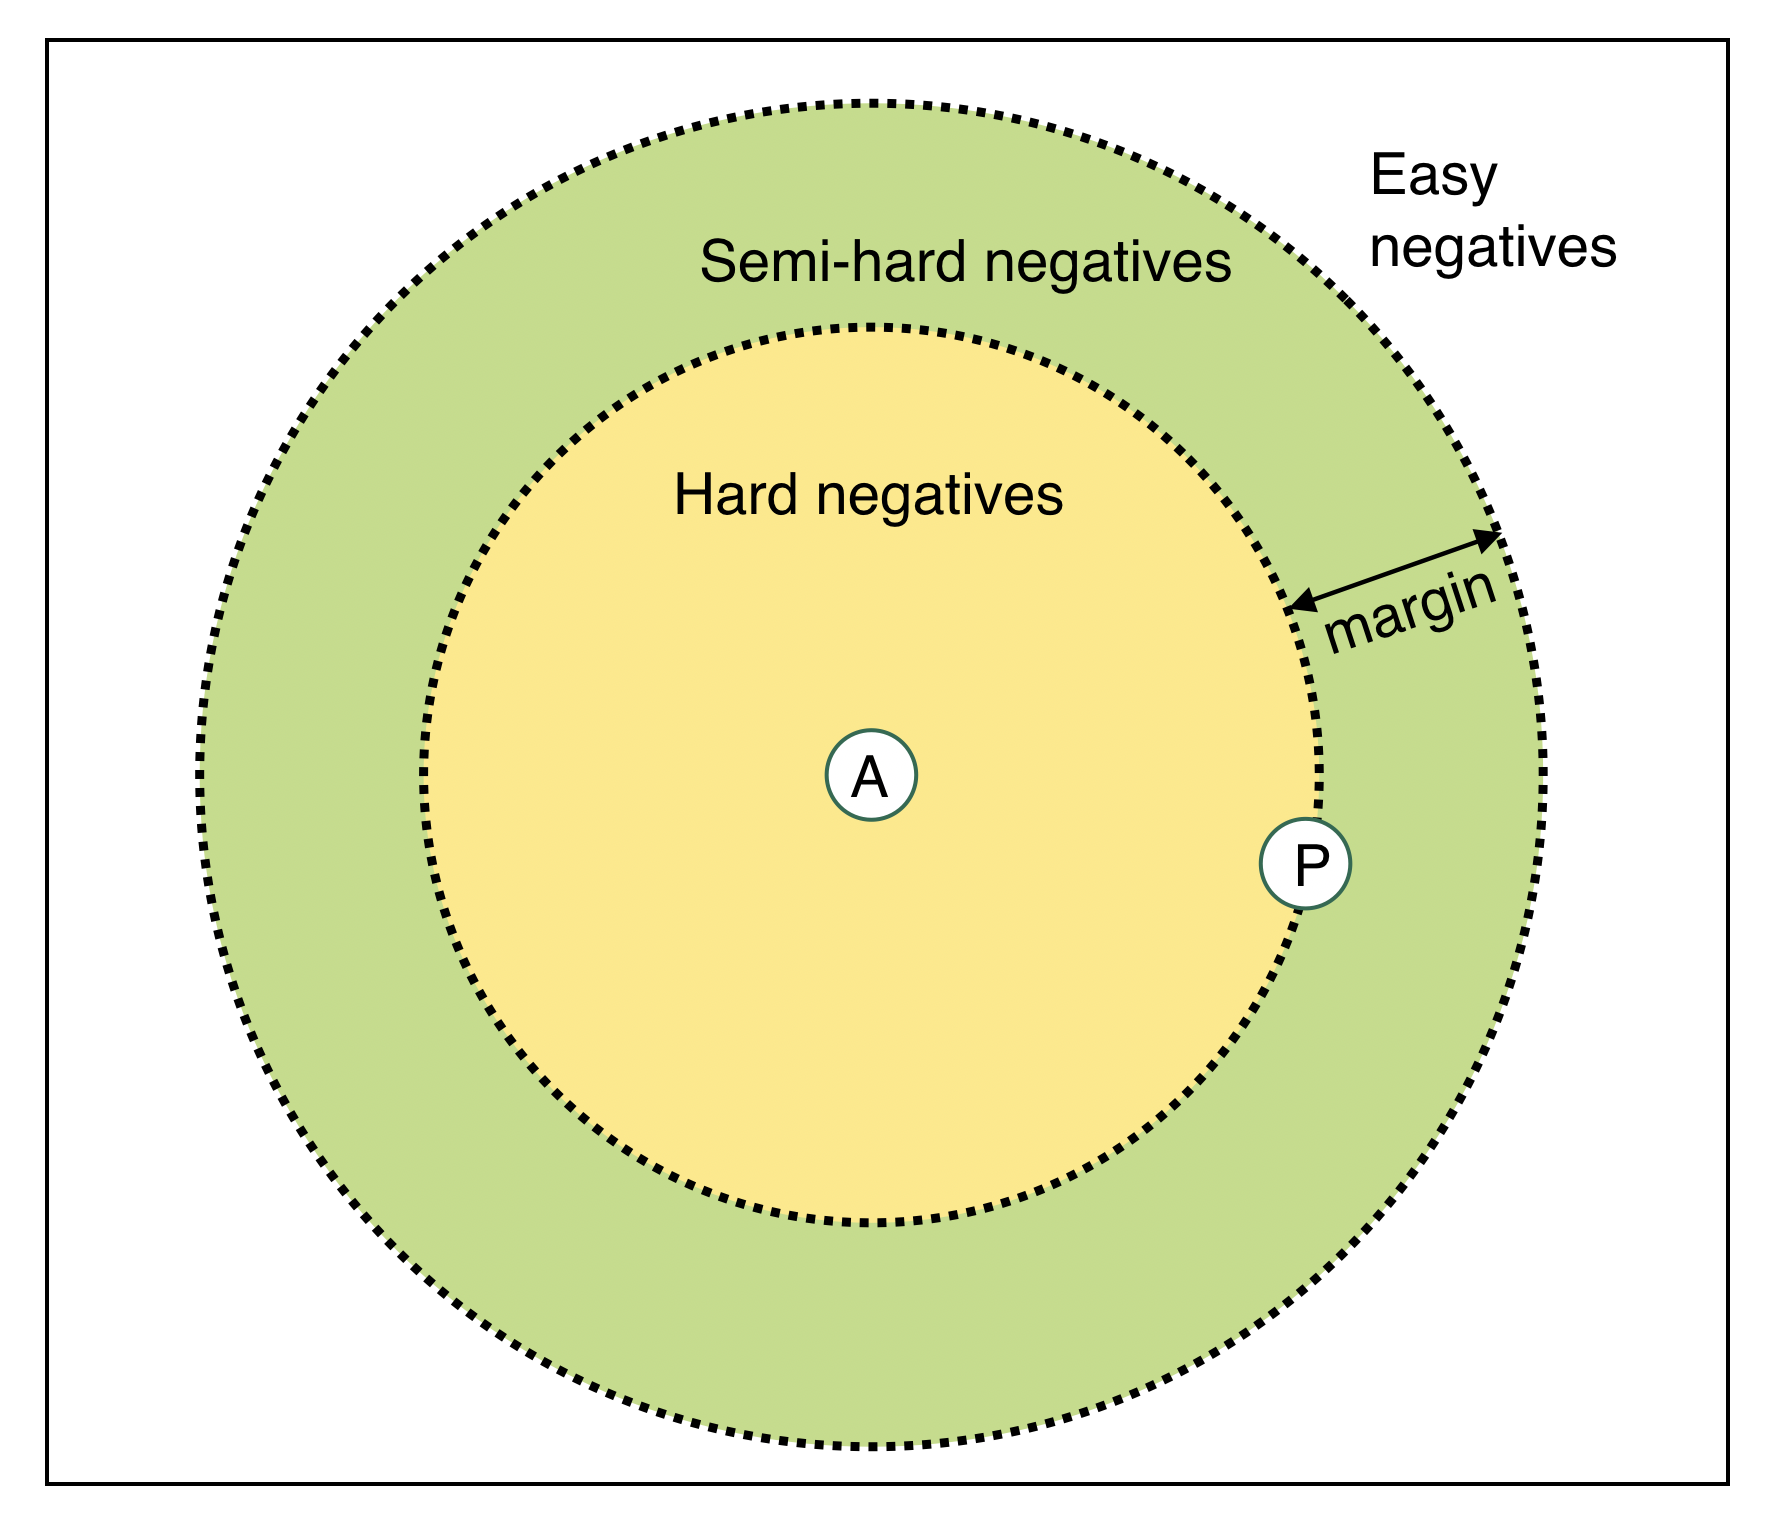
\includegraphics[width=0.6\linewidth]{figs/sitiations.png}
  \caption{Three situations of triplet loss.}
  \label{fig:sitiations}
\end{figure}






\section{Evaluation}

\subsection{Implementation of Transfer Learning}

\subsection{Implementation of Siamese Network}

In this project, we implement both two loss functions with the same dataset. The dataset processing is presented in section \ref{}. 

\subsubsection{Implementation of contrastive loss}
For contrastive loss, we implement and train siamese networks using Keras and Tensorflow. The implementation can be partitioned into three steps: 1) generating image pairs, 2) construct the architecture of the siamese neural network, 3) using contrastive loss to train the model. Note that the siamese network was designed originally for the image matching task, not the image classification. Normally, it would have a distance function to compute the similarity between the two embedding vectors as the final outputs. However, our project is for the image classification problem, so we implement a single dense layer on top of that to train the embedding vectors extracted from the siamese network. In doing so, we get classification results that are similar to the transfer learning models. 

Specifically, in this project, we adopt a simple strategy to make the image pairs. The positive sample of an anchor sample is picked randomly from the same category as the anchor. On the other hand, we grab the negative sample randomly from classes that are different from the one that the anchor belongs to. Furthermore, we label the positive pairs with 1 and the positive pairs with 0. Figure \ref{fig:threesamples} shows the examples of the anchor, positive and negative samples. 

\begin{figure}[h]
  \centering
  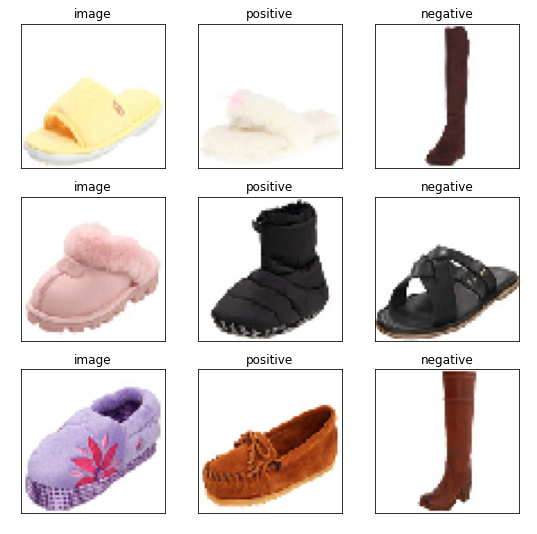
\includegraphics[width=0.9\linewidth]{figs/threesamples.png}
  \caption{Examples of anchor, positive and negative samples.}
  \label{fig:threesamples}
\end{figure}

Furthermore, we can also compute the similarity between image pairs, as shown in figure \ref{}. Note that the smaller distance between the two images means they are more similar to each other. For example, in the figure, the distance between the first pair is 0.12, and it turns out that they belong to the same class Slippers. As for the second pair, the class of left image is Slippers and the class of right image is Sandals. The distance between them is 0.56, which is much larger than the first pair, as we expected. 

\begin{figure}[h]
  \centering
  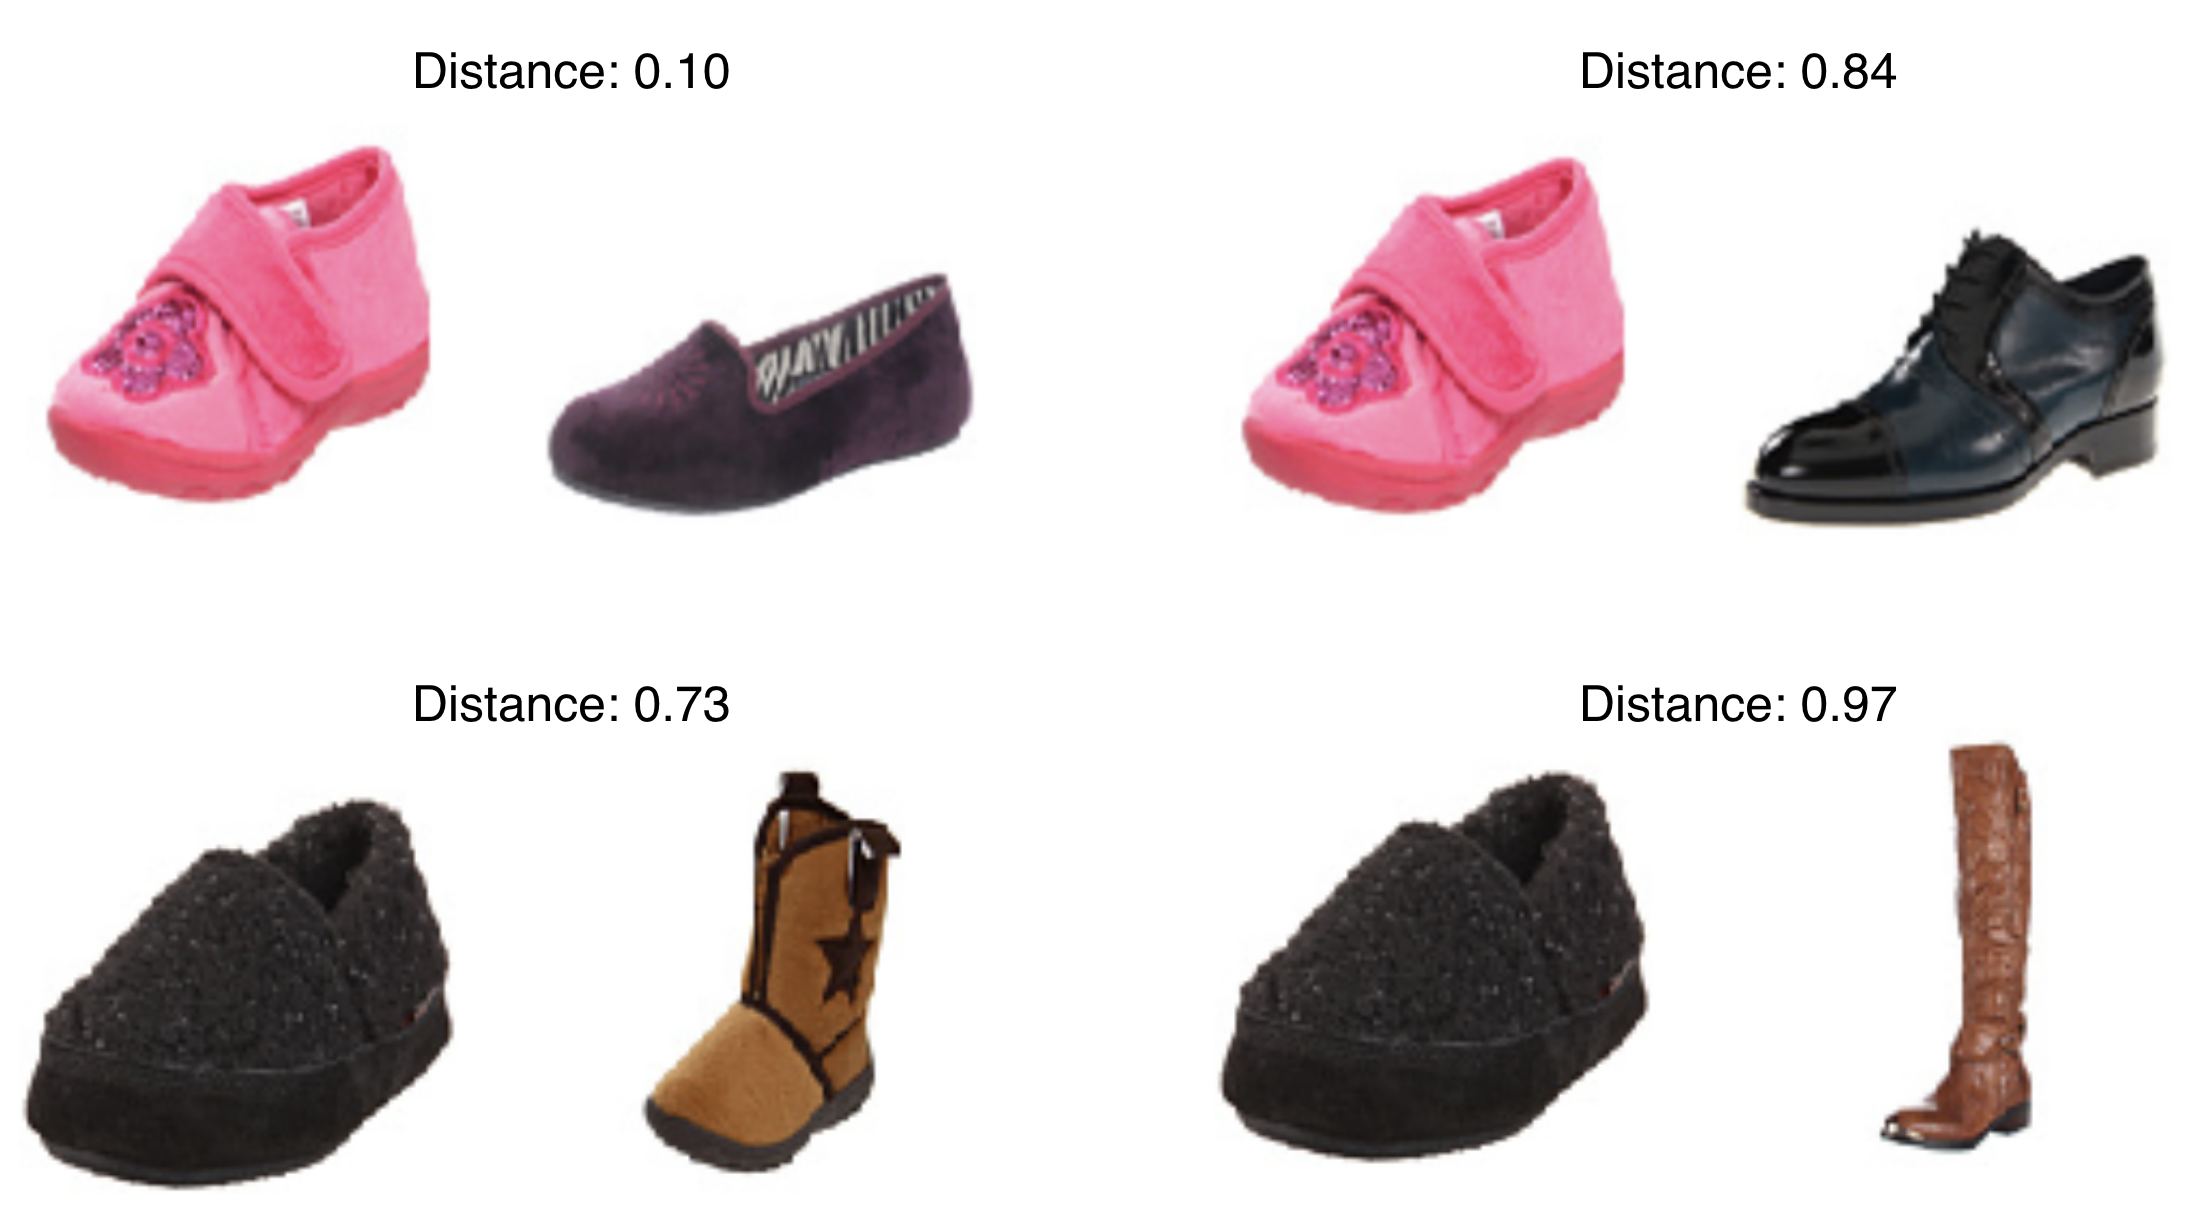
\includegraphics[width=0.5\linewidth]{figs/similarity.png}
  \caption{Examples of calculating the similarity of image pairs.}
  \label{fig:similarity}
\end{figure}

\subsubsection{Implementation of triplet loss}


\subsection{Comparison and Analysis}

In our implementation, we observe that the triplet loss a little outperforms the contrastive loss. The possible reasons could be the triplet loss tries to be less greedy than contrastive loss since the distance is a relative concept. The triplet loss tries to bring the positive sample closer while also pushing away the negative sample when compared with an anchor, as shown in the figure \ref{fig:tripletloss}. In doing so, the model can clear know if the distance between the anchor sample and positive sample is smaller than the distance between the anchor and negative one. On the other hand, the contrastive loss, only considers one pair at a time, either positive or negative, so in a sense, it is more greedy. It's hard to ensure the similar objects are close enough. 

\begin{figure}[h]
  \centering
  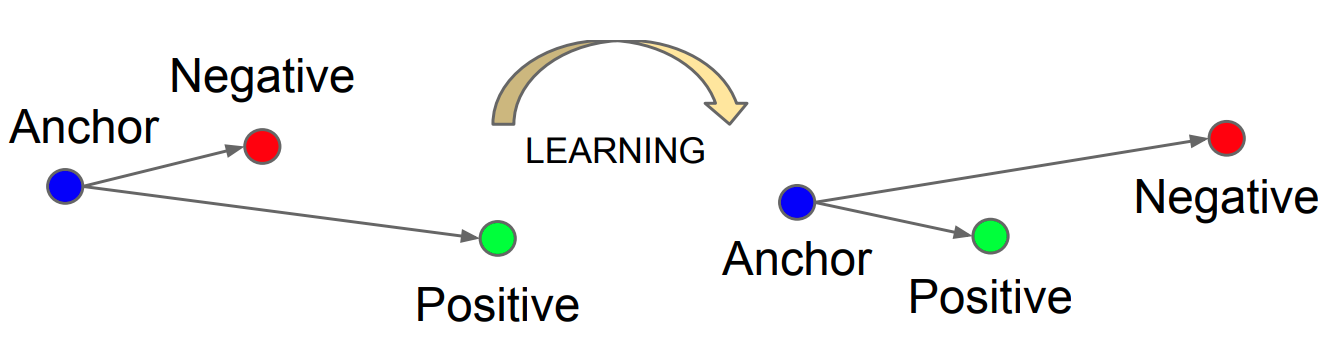
\includegraphics[width=\linewidth]{figs/tripletloss.png}
  \caption{The Triplet Loss minimizes the distance between an anchor and a positive, and maximizes the distance between the anchor and a negative.}
  \label{fig:tripletloss}
\end{figure}



%%
%% The next two lines define the bibliography style to be used, and
%% the bibliography file.
\bibliographystyle{ACM-Reference-Format}
\bibliography{dl21}
%%
%% If your work has an appendix, this is the place to put it.
%\appendix

\end{document}
\endinput
%%
%% End of file `sample-sigconf.tex'.
